% !Mode:: "TeX:UTF-8"
\chapter{基因表达数据的双聚类相关概述}

\section{基因表达数据}
  数据的好坏在很大程度上决定了结果的好坏。基因表达数据主要通过基因芯片技术和下一代测序技术等这些高通量基因表达测量技术获得。这些技术可以同时在不同的样本或条件下,对成千上万的基因进行高效、精确、定量地测量。这时只是得到了一些原始数据,由于在特定条件下只有很少数的基因会表达,里面会存在很多缺失数据。需要对原始数据进行缺失值和去噪处理,才能得到适合数据挖掘的数据。

  基因表达数据极其庞大,以及需要专业的生物知识,导致很多跨领域的研究者很难涉足。为了打破这种学科壁垒,科学家们提出了关于描述和存储基因表达数据的标准,并在标准之上建立了基因表达数据库。最广泛的数据库为GEO(Gene Expression Omnibus),由美国国家生物技术信息中心于2000年开发。该数据库提供了共享基因表达数据的平台,并且有专业的人员进行审核。公共数据库的出现,极大促进了生物信息学的发展。

  基因表达数据一般以一个二维矩阵\textit{E}表示,一行代表一个基因,一列代表一个实验条件。实验条件包括不同时期,不同组织,不同个体,不同外部环境等等。矩阵\textit{E}中的每个元素$e_{ij} $表示基因$g_i$在实验条件$c_j$下的表达水平值,其生物含义是该基因在此条件下,细胞中mRNA的含量。

\section{双聚类的相关概念}

  \subsection{双聚类的定义}
  给定一个大小为$n\times m$基因表达数据$\textit{E(X,Y)}$,假定集合$I\subseteq X,(|I| = k \leq n)$是\textit{E}的基因集合$X$的子集;集合$J\subseteq Y,(|J| = l \leq m)$是\textit{E}的基因集合$Y$的子集。如图\ref{fig:define_bic}所示,双聚类是指在条件子集$J$下的基因表达模型表现出同源特性的基因子集$I$。因此,双聚类可以定义为一个$k \times l$的子矩阵$B(I, J)$,也简称为$B$。
  \begin{figure}[htbp]
      \centering
  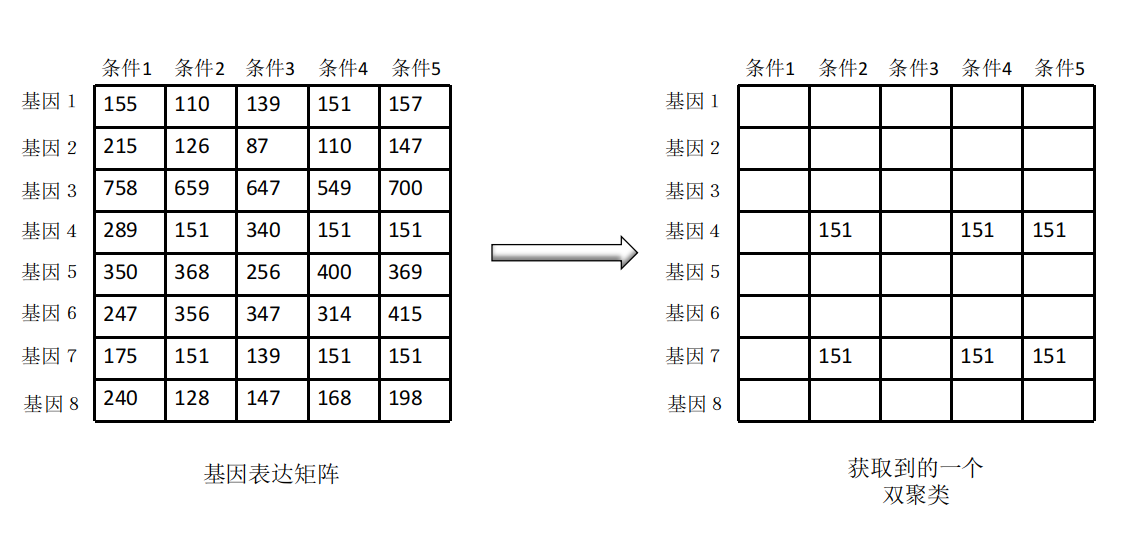
\includegraphics[width = 0.8\textwidth]{aBicluster.png}
  \caption{双聚类定义示例}
  \label{fig:define_bic}
  \end{figure}

  \subsection{双聚类的类型}
    给定一个二维矩阵$A(I,J)$,$a_{ij}$为其中第$i$行第$j$列的值,$\alpha_i$是一个与行有关而与列无关的变量,$\beta_j$是一个与列有关而与行无关的变量,$0\le h,r,t,d \le |I|$或$0\le h,r,t,d \le |J|$。Madeira 和 Oliveira提出,在双聚类中主要有以下四种结构:
    \begin{enumerate}
        \item[1.] 具有相同常量值的双聚类,如图\ref{bic61}所示,公式如下。
        \begin{equation}
         a_{ij}=\mu
        \end{equation}

        \item[2.] 列或行具有相同常量值的双聚类,如图\ref{bic62}和\ref{bic63}所示,公式如下。 
        \begin{equation}
        (a_{ij}=\mu+\alpha_i \mbox{或} a_{ij}=\mu *\alpha_i)  
        \mbox{且}
        (a_{ij}=\mu+\beta_j \mbox{或} a_{ij}=\mu *\beta_j)
        \end{equation}
        
        \item[3.] 具有连贯值的双聚类,如图\ref{bic64}和\ref{bic65}所示,公式如下。
        \begin{equation}
        a_{ij}=\mu+\alpha_i+\beta_j \mbox{或} a_{ij}=\mu *\alpha_i*\beta_j
        \end{equation} 

        \item[4.] 具有连贯演变的双聚类,如图\ref{bic66}所示,公式如下。
        \begin{equation}
        a_{ih}\le a_{ir}\le a_{it}\le a_{id} \mbox{或} a_{hj}\le a_{rj}\le a_{tj}\le  a_{dj} 
        \end{equation}
    \end{enumerate}
    则双聚类可以根据相对应的的结构分类。根据要解决问题的特定属性,需要考虑不同结构的双聚类。

  \begin{figure}[!h]
  \setlength{\subfigcapskip}{-1bp}
  \centering
  \begin{minipage}{.7\textwidth}
  \centering
  \subfigure{\label{bic61}}\addtocounter{subfigure}{-2}
  \subfigure{\subfigure[]{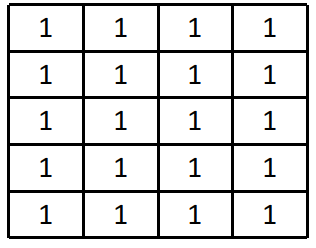
\includegraphics[width=0.3\textwidth]{a-bic}}}
  \hspace{.2em}
  \subfigure{\label{bic62}}\addtocounter{subfigure}{-2}
  \subfigure{\subfigure[]{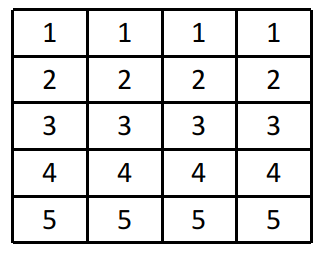
\includegraphics[width=0.3\textwidth]{b-bic}}}
  \hspace{.2em}
  \subfigure{\label{bic63}}\addtocounter{subfigure}{-2}
  \subfigure{\subfigure[]{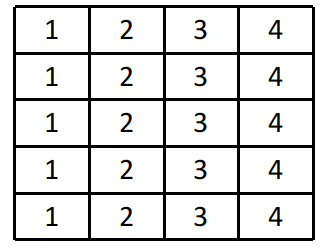
\includegraphics[width=0.3\textwidth]{c-bic}}}
  \end{minipage}
  \centering
  \begin{minipage}{.7\textwidth}
  \centering
  \subfigure{\label{bic64}}\addtocounter{subfigure}{-2}
  \subfigure{\subfigure[]{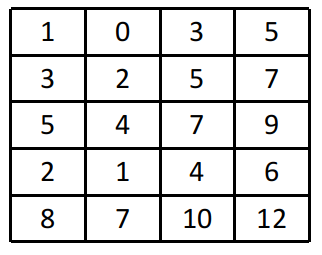
\includegraphics[width=0.3\textwidth]{d-bic}}}
  \hspace{.2em}
  \subfigure{\label{bic65}}\addtocounter{subfigure}{-2}
  \subfigure{\subfigure[]{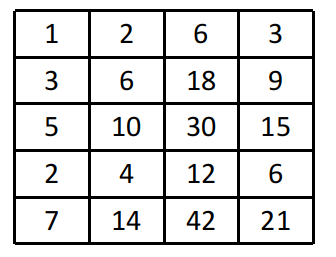
\includegraphics[width=0.31\textwidth]{e-bic}}}
  \hspace{.2em}
  \subfigure{\label{bic66}}\addtocounter{subfigure}{-2}
  \subfigure{\subfigure[]{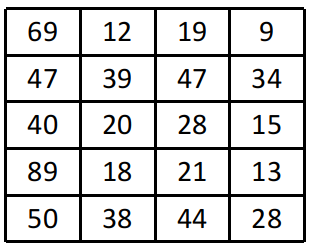
\includegraphics[width=0.3\textwidth]{f-bic}}}
  \end{minipage}
  \vspace{0.2em}
  \caption{双聚类的类型}
  \end{figure}

  \subsection{双聚类的结构}
  双聚类的结构是指,通过算法找到的双聚类之间在原始矩阵时间的相对位置。根据结构,大体可以分为8类,如下图所示:
  \begin{figure}[!h]
  \setlength{\subfigcapskip}{-1bp}
  \centering
  \begin{minipage}{.8\textwidth}
  \centering
  \subfigure{\label{bic81}}\addtocounter{subfigure}{-2}
  \subfigure{\subfigure[单一双聚类结构]{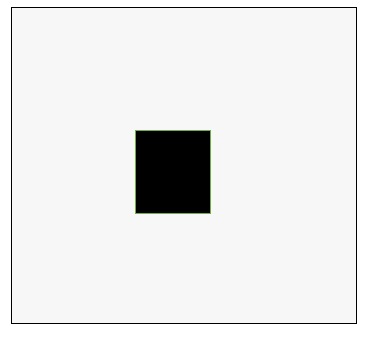
\includegraphics[width=0.2\textwidth]{struct1}}}
  \hspace{.2em}
  \subfigure{\label{bic82}}\addtocounter{subfigure}{-2}
  \subfigure{\subfigure[对角结构]{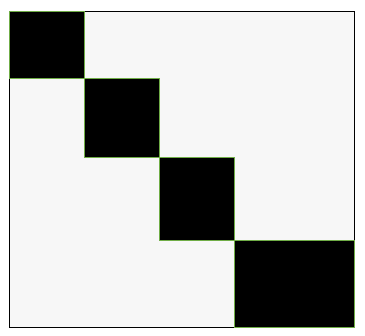
\includegraphics[width=0.2\textwidth]{struct2}}}
  \hspace{.2em}
  \subfigure{\label{bic83}}\addtocounter{subfigure}{-2}
  \subfigure{\subfigure[棋盘结构]{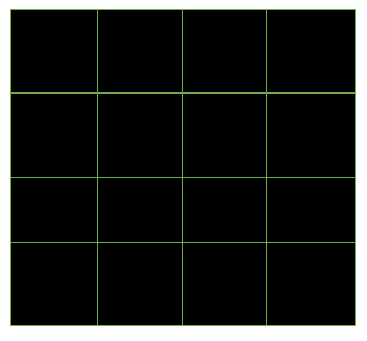
\includegraphics[width=0.2\textwidth]{struct3}}}
  \hspace{.2em}
  \subfigure{\label{bic84}}\addtocounter{subfigure}{-2}
  \subfigure{\subfigure[行互斥结构]{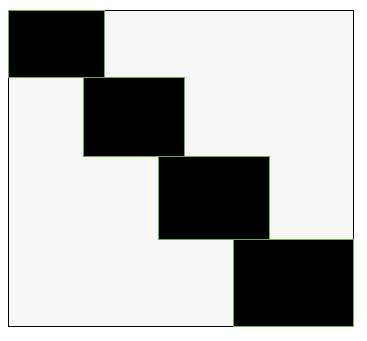
\includegraphics[width=0.2\textwidth]{struct4}}}
  \end{minipage}
  \centering
  \begin{minipage}{.8\textwidth}
  \centering
  \hspace{.2em}
  \subfigure{\label{bic85}}\addtocounter{subfigure}{-2}
  \subfigure{\subfigure[列互斥结构]{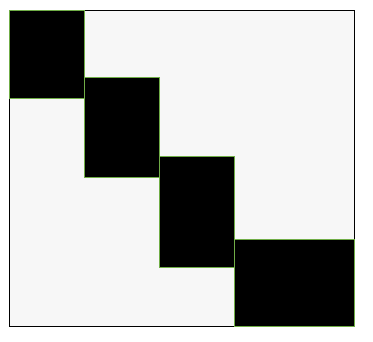
\includegraphics[width=0.2\textwidth]{struct5}}}
  \hspace{.2em}
  \subfigure{\label{bic86}}\addtocounter{subfigure}{-2}
  \subfigure{\subfigure[非互斥且非重叠结构]{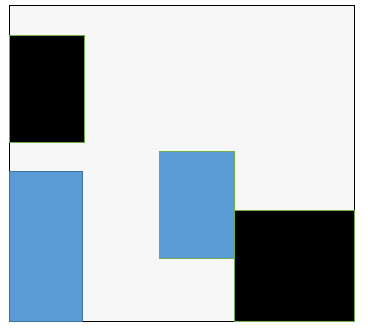
\includegraphics[width=0.2\textwidth]{struct6}}}
  \hspace{.2em}
  \subfigure{\label{bic87}}\addtocounter{subfigure}{-2}
  \subfigure{\subfigure[嵌套重叠结构]{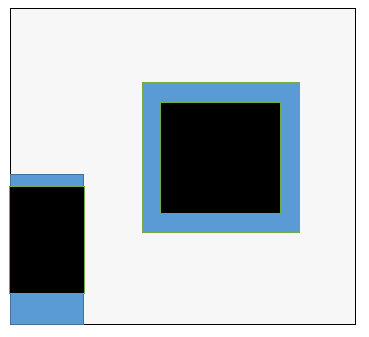
\includegraphics[width=0.2\textwidth]{struct7}}}
  \hspace{.2em}
  \subfigure{\label{bic88}}\addtocounter{subfigure}{-2}
  \subfigure{\subfigure[任意重叠结构]{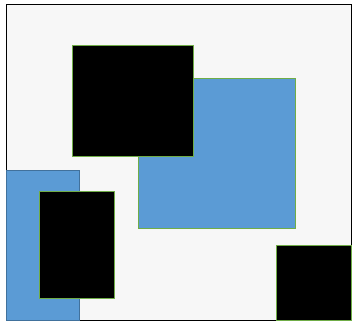
\includegraphics[width=0.2\textwidth]{struct8}}}
  \end{minipage}
  \vspace{0.2em}
  \caption{双聚类的结构}
  \end{figure}

% \section{双聚类算法的分类}

%   \subsection{基于质量评价指标的双聚类算法}

%   \subsection{基于模型的双聚类算法}

  
\section{双聚类的验证指标}
  \subsection{质量验证指标}

  \subsection{生物验证指标}

\section{群智能算法}

    目前,有很多优秀的优化算法,有确定性方法如线性规划、二次规划,动态规划和梯度下降;以及随机性方法如群体智能。这些方法让我们能够在一定的时间内解决某些问题。然而,处理大量高维数据时,确定性方法太过复杂导致需要大量的计算成本。元启发式的群体智能算法因其高效率越来越受到关注。

  \subsection{布谷鸟搜索算法}
    布谷鸟搜索算法(Cuckoo Search, CS)是Yang和Deb于2009年提出的新兴启发算法。该算法通过模拟布谷鸟寄生育雏行为,在可行域中通过Levy飞行寻找合适的鸟巢,来找到较优解。该算法有三条理想化的规则:
    \begin{enumerate}
      \item {每只布谷鸟每次下一个蛋,并将其放入随机选择的巢中。}
      \item {具有优质蛋的最佳巢会被带到下一代。}
      \item {可用的寄主巢数量是固定的,且寄主以概率$P_a\in(0,1)$发现布谷鸟放的蛋。在这种情况下,寄主可以消灭该蛋或放弃旧巢另建新巢。}
    \end{enumerate}

    CS中有两种更新方式,一种是布谷鸟寻找宿主鸟巢的Levy飞行:
    \begin{align}
      x_{i+1}=x_i+\alpha\otimes Levy(\beta)
    \end{align}
    其中,$\alpha$是步长缩放因子, $Levy(\beta)$是Levy飞行路径。

    另一种是寄主以概率$P_a$发现外来鸟蛋后,采用随机方式重新建巢:
    \begin{equation}
      x_{i+1}=x_i+r\otimes Heaviside(P_a-\varepsilon)\otimes(x_t-x_k)
    \end{equation}
    其中,$r,\varepsilon$是服从均匀分布的随机数,$Heaviside()$是跳跃函数,$x_t,x_k$是其他任意的两个鸟巢。

  \subsection{萤火虫算法}
    萤火虫算法(Firefly Algorithm,FA)是Yang于2008年提出的一种启发算法。把空间各点看成萤火虫,利用发光强的萤火虫会吸引发光弱的萤火虫的特点,在发光弱的萤火虫向发光强的萤火虫移动的过程中,完成位置的迭代,从而找出最优位置。算法有以下三条假设:
    \begin{enumerate}
      \item {萤火虫不分性别,这样一个萤火虫将会吸引到所有其他的萤火虫。}
      \item {吸引力与它们的亮度成正比,对于任何两个萤火虫,不那么明亮的萤火虫被吸引,因此移动到更亮的一个,然而,亮度又随着其距离的增加而减少。}
      \item {如果没有比一个给定的萤火虫更亮的萤火虫,它会随机移动。}
    \end{enumerate}
    萤火虫的相对荧光亮度计算方式:
    \begin{align}
      I=I_0e^{-\gamma r_{ij}}
    \end{align}
    其中, $I_0$表示最亮萤火虫的亮度,即自身($r=0$处)荧光亮度,与目标函数值相关,目标函数值越优,自身亮度越高;$\gamma$表示光吸收系数,因为荧光会随着距离的增加和传播媒介的吸收逐渐减弱,所以设置光强吸收系数以体现此特性,可设置为常数;$r_{ij}$表示萤火虫$i$与$j$之间的距离。 

    当萤火虫$i$的相对亮度小于萤火虫$j$时,向萤火虫$j$靠拢。位置的更新方式为:
    \begin{align}
      \beta(r)&=\beta_0e^{-\gamma r_{ij}^2} \\
      x_i&=x_i+\beta(x_j-x_i)+\alpha(rand-1/2)
    \end{align}
    其中, $\beta_0$表示最大吸引度,即光源处($r=0$处)的吸引度。$\alpha$为步长因子,$rand$为[0,1]上服从均匀分布的随机因子。

  \subsection{细菌觅食算法算法}
  细菌觅食算法算法(Bacterial Foraging Optimization,BFO)由Passino于2002年提出。通过模拟大肠杆菌菌落的觅食行为,不断地使用鞭毛游动和翻转,最终躲开有毒的地方并找到营养度高的位置,如图\ref{fig:bfo}所示。算法分为趋向性操作、复制操作和迁徙操作。
  \begin{figure}[htbp]
    \centering
    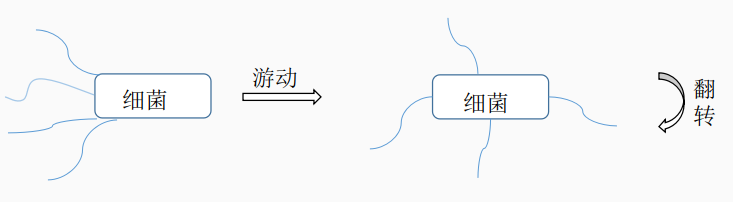
\includegraphics[width = 0.7\textwidth]{bfo.png}
    \caption{细菌的游动和翻转}
    \label{fig:bfo}
  \end{figure}

  \begin{enumerate}
    \item[1.] 趋向性操作。 
    这一操作模拟得是大肠杆菌的游动和翻转。在营养度高的地区,细菌会更多地游动,在营养度低的地区,细菌会更多地翻转,以逃出该地区。设细菌的种群规模为$S$,维度为$n$。细菌的觅食行为可以用以下公式表示:
    \begin{align}
      \theta(i,j+1,k,l) &= \theta(i,j,k,l) + C(i) \times \phi(i,j) \\
      \phi(i,j) &= \frac{\Delta(i)}{\sqrt{\Delta^T(i)\Delta(i)}}
    \end{align}
    其中,$\theta(i,j,k,l)$表示细菌在第$j$次趋向性操作,第$k$次复制操作和第$l$次迁徙操作时的位置。$C(i)$是细菌$i$的趋向性步长。$\phi(i,j)$表示细菌在第$j$次趋向性操作时的随机方向的单位向量。$\Delta(i)$为随机向量。

    \item[2.] 复制操作。
    复制操作的目的是将表现不好的细菌淘汰掉。首先,对种群按适应度排序,然后,前一半的细菌会复制一份覆盖后一半的细菌。保持种群数量不变的同时,实现优胜劣汰的机制。

    \item[3.] 迁徙操作。
    在生物观察中发现,随着某些条件的改变,可能会使该地区的细菌突然死亡或迁移。算法通过迁徙操作模拟这一现象,提高种群的多样性。细菌会以一定的概率被清除,并随机生成一个新的细菌。
    
  \end{enumerate}

\section{本章小结}